\documentclass[../../main.tex]{subfiles}
\begin{document}

\parpic[r]{
    \begin{linearEquation}
        %Füllung linke Waagschale
        \node[white,marble,inner sep=.12cm] at (-1,0.4) {$x$};
        %Füllung rechte Waagschale
        \fill (0.75,0.25) -- (1.25,0.25) -- (1.2,0.65) -- (0.8,0.65) -- cycle;
        \draw[line width=0.75mm] (1,0.71) circle[radius=0.06cm];
        \node[white] at (1,0.45) {$56$};
    \end{linearEquation}
}
In den Kapiteln über \hyperlink{chap:lineare_gleichungen}{\emph{Lineare Gleichungen}} und \hyperlink{chap:lgs}{\emph{Lineare Gleichungssysteme}} 
hast du bereits herausgefunden, wie du lineare Gleichungen und Gleichungssysteme mit
Äquivalenzumformungen lösen kannst. Kommt in der Gleichung zum Beispiel wie rechts die \emph{Unbekannte} $x$ vor, 
so ist deine Aufgabe, mögliche Werte zu bestimmen, die du für $x$ einsetzen kannst, damit die Gleichung erfüllt ist.

Dafür müssen wir sie in einer Gleichung \emph{isolieren}, sodass sie (wie rechts abgebildet) allein auf einer Seite der 
Gleichung steht. Dieses Ziel können wir bei 
linearen Gleichungen immer durch einfache Äquivalenzumformungen erreichen (siehe Seite 
\pageref{lineare-gleichungen-loesungsverfahren}). Haben wir anschließend etwa die Gleichung
\[x=56,\]
so lässt sich der Wert von $x$ sofort als $56$ ablesen. Leider ist die Einschränkung, dass eine Gleichung linear
sein muss, damit wir sie lösen können, sehr stark und bereits bei vielen einfacheren Problemen bringen uns lineare
Gleichungen nicht zum Ziel.
\begin{example}{}
    Stell dir vor, du möchtest dir ein paar Kaninchen zulegen und ih

    Wenn du die Klammer auflöst, erhältst du die Gleichung $x^2-2x=143$. Diese Gleichung ist nicht linear, weil auf
    der linken Seite der Term $x^2$ vorkommt. Diesen Term können wir nicht durch Termumformungen loswerden.
\end{example}
Eine Gleichung ist nur dann linear, wenn sie sich durch Termumformung in eine ganz bestimmte Form bringen lässt, in der
links und rechts jeweils Terme wie in der folgenden Gleichung stehen.
\[2x+4=7x-9.\]
Dabei sind die genauen Zahlen natürlich beliebig. Nicht linear ist hingegen die Gleichung
\[x^2+9=25,\]
denn auf der linken Seite steht der Term $x^2$, der in linearen Gleichungen nicht erlaubt ist. In diesem Kapitel 
erlauben wir auch Gleichungen, bei denen auf der linken oder rechten Seite zusätzlich der Term $x^2$ vorkommt -- ggf. 
mit Vorfaktor. Eine solche Gleichung nennen wir
\textbf{quadratische Gleichung}, denn der Wert $x$ kommt nun auch quadriert vor. Die Gleichung $x^2+9=25$ ist ein 
Beispiel für eine quadratische Gleichung.

\begin{example}[ex:normalform-quadratische-gleichung]{}
    Die Gleichung $4x^2+7x+16=3x^2-x$ ist eine quadratische Gleichung. Sie unterscheidet sich von linearen Gleichungen
    nur dadurch, dass links zusätzlich noch der Term $4x^2$ und rechts der Term $3x^2$ steht. 
    
    Wir vereinfachen die
    Gleichung ein wenig, indem wir mit Äquivalenzumformungen alle Terme von rechts auf die linke Seite schieben:
    \begin{align*}
        4x^2+7x+16&=3x^2-x\commentLine{+x}\\
        4x^2+8x+16&=3x^2\commentLine{-3x^2}\\
        x^2+8x+16&=0
    \end{align*}
    Das Ergebnis ist eine quadratische Gleichung, bei der nur noch auf einer Seite vom Gleichheitszeichen Werte stehen,
    die nicht 0 sind. Das ist kürzer als eine Gleichung, bei der auf beiden Seiten ein längerer Term steht. Da wir
    eine quadratische Gleichung immer so umformen können, dass rechts eine 0 steht, werden wir uns in Zukunft Zeit 
    sparen, indem wir davon ausgehen, dass wir immer mit einer solchen Gleichung starten.
\end{example}

Quadratische Gleichungen lassen sich natürlich ebenso wie jede andere Gleichung auch mit Äquivalenzumformungen umformen.
Dabei ist es immer möglich, die Gleichung so umzuformen, dass rechts vom Gleichheitszeichen eine 0 steht (siehe 
Beispiel \ref{ex:normalform-quadratische-gleichung}). Übrig bleibt
ein Term auf der linken Seite der Gleichung, den wir als $ax^2+bx+c$ schreiben können, wenn wir für $a,b$ und $c$ 
passende Zahlen wählen. Die Gleichung lautet dann
\[ax^2+bx+c=0.\]
\begin{example}{}
    In der Gleichung $2x^2-8x+11=0$ lässt sich die linke Seite als $ax^2+bx+c$ schreiben, wenn wir $a=2, b=-8$ und 
    $c=11$ wählen.
\end{example}

\begin{definition}{Quadratische Gleichung}
    Eine \textbf{quadratische Gleichung} ist eine Gleichung, die sich durch Äquivalenzumformungen in die Form
    \[ax^2+bx+c=0\]
    mit $a,b,c\in\R$ und $a\neq 0$ bringen lässt.
\end{definition}
\subsection*{Lösungsverfahren für einfachere Sonderfälle}
Unser Ziel ist es nun, zu untersuchen, wie sich quadratische Gleichungen auflösen lassen. Dafür schauen wir uns in
diesem Abschnitt erstmal ein paar Sonderfälle an, in denen wir gut mit den Äquivalenzumformungen aus dem Kapitel über
lineare Gleichungen zum Ziel kommen. Im nächsten Abschnitt entwickeln wir dann ein allgemeines Lösungsverfahren.
\begin{example}{}
    \parpic[r]{
        \begin{linearEquation}
            %Füllung linke Waagschale
            \node[white,marble,inner sep=.12cm] at (-1.2,0.4) {$x^2$};
            \fill (-1.05,0.25) -- (-0.65,0.25) -- (-0.7,0.6) -- (-1,0.6) -- cycle;
            \draw[line width=0.75mm] (-0.85,0.66) circle[radius=0.06cm];
            \node[white] at (-0.85,0.42) {$6$};
            %Füllung rechte Waagschale
            \fill (0.75,0.25) -- (1.25,0.25) -- (1.2,0.65) -- (0.8,0.65) -- cycle;
            \draw[line width=0.75mm] (1,0.71) circle[radius=0.06cm];
            \node[white] at (1,0.45) {$31$};
        \end{linearEquation}
    }
    \picskip{8}
    Rechts siehst du die Gleichung $x^2+6=31$ -- dargestellt als Balkenwaage. Diese Gleichung sieht ähnlich aus wie
    die lineare Gleichung $x+6=31$ -- nur mit dem Unterschied, dass anstelle des $x$ nun ein $x^2$ auf der linken Seite
    steht. Deshalb haben wir im Bild wieder eine Balkenwaage verwendet, wie du sie aus dem Kapitel über lineare
    Gleichungen kennst und die Kugel einfach mit $x^2$ beschriftet.

    Nun versuchen wir, die Gleichung genau so aufzulösen wie wir es bereits kennen: Die Kugel soll am Ende allein auf
    der linken Seite liegen, damit wir rechts ihr Gewicht ablesen können. Oder mathematisch: Der Term $x^2$ soll allein
    auf der linken Seite stehen. Dafür müssen wir das Gewicht mit der 6 von der Waage entfernen (und das gleiche auch
    rechts machen, weil die Waage sonst links leichter wäre und kippen würde). Wir subtrahieren also auf beiden Seiten
    6 und bekommen
    \begin{align*}
        x^2+6&=31\commentLine{-6}\\
        x^2&=25.
    \end{align*}
    Wenn wir es mit einer linearen Gleichung zu tun gehabt hätten, dann wären wir jetzt fertig. Leider verrät uns diese
    Gleichung jetzt aber noch nicht den Wert von $x$, sondern nur den Wert von $x^2$. Wenn $x^2=x\cdot x$ den Wert 25
    haben soll, dann suchen wir folglich einen Wert für $x$, der mit sich selbst multipliziert 25 ergibt.

    Glücklicherweise kennen wir bereits einen Weg, hier weiter zu rechnen: Die \emph{Wurzel} einer Zahl $a$ ist die Zahl, 
    die mit sich selbst 
    multipliziert werden muss, um $a$ zu erhalten. Zum Beispiel ist $\sqrt{25}=5$, denn $5\cdot 5=25$. Damit haben wir 
    mit $x=5$ eine Lösung unserer Gleichung gefunden.
\end{example}

Schauen wir uns zunächst ein paar quadratische Gleichungen an, die zwar Terme mit $x^2$ 
enthalten, aber keinen Term, in dem das $x$ ohne Quadrat vorkommt -- etwa die Gleichung $2x^2+3=19+x^2$.
Solche Gleichungen können wir auflösen, indem wir zunächst so tun als hätten wir es mit einer linearen
Gleichung zu tun, die wir nach der Unbekannten $x^2$ auflösen möchten. Anschließend können wir durch Wurzelziehen an den
Wert von $x$ kommen. Wir schauen uns dieses Vorgehen gleich etwas genauer an. Vorher müssen wir allerdings sicherstellen,
dass dass wir beim Wurzelziehen keine Lösungen \enquote{vergessen}.

\begin{example}{Es gibt zwei Lösungen!}
    Aus dem Kapitel über \hyperlink{ch:ganze-zahlen}{ganze Zahlen} kennst du die Regel, dass das Produkt zweier
    negativer Zahlen positiv ist (\enquote{Minus mal Minus ist Plus}). Es wäre also nicht aufgefallen, wenn du eben 
    statt $5\cdot 5$ einfach $(-5)\cdot (-5)$ gerechnet hättest, denn das Ergebnis dieser Rechnung ist ebenfalls 25.

    Die Gleichung $x^2=25$ ist also \emph{nicht} äquivalent zur Gleichung $x^2=5$, weil die erste Gleichung auch durch
    $x=-5$ gelöst wird, die zweite aber nicht. Stattdessen ist die Gleichung $x^2=25$ äquivalent zu
    \[x=5\text{ oder }x=-5.\]
\end{example}

\textbf{Schritt 1: Gleichung aufstellen und vereinfachen}
\parpic[r]{
    \begin{linearEquation}
        %Füllung linke Waagschale
        \node[white,marble,inner sep=.1cm] at (-1,0.4) {\small $x^2$};
        \fill (-1.5,0.25) -- (-1.1,0.25) -- (-1.15,0.6) -- (-1.45,0.6) -- cycle;
            \draw[line width=0.75mm] (-1.3,0.66) circle[radius=0.06cm];
            \node[white] at (-1.3,0.42) {$3$};
        \node[white,marble,inner sep=.1cm] at (-0.65,0.4) {\small $x^2$};
        %Füllung rechte Waagschale
        \node[white,marble,inner sep=.1cm] at (0.8,0.4) {\small $x^2$};
        \fill (1,0.25) -- (1.5,0.25) -- (1.45,0.65) -- (1.05,0.65) -- cycle;
            \draw[line width=0.75mm] (1.25,0.71) circle[radius=0.06cm];
            \node[white] at (1.25,0.45) {$19$};
    \end{linearEquation}
}
Wenn du es mit einer Textaufgabe zu tun hast, musst du zunächst eine Gleichung aufstellen, die du lösen kannst. Bevor du
beginnst, die Gleichung zu lösen, versuche zunächst, die beiden Seiten der Gleichung durch Termunformung möglichst weit
zu \textbf{vereinfachen}. Anschließend erhältst du zum Beispiel die Gleichung
\[3+2x^2=19+x^2.\]

\textbf{Schritt 2: Wie eine lineare Gleichung auflösen}
\parpic[r]{
    \begin{linearEquation}
        %Füllung linke Waagschale
        \node[white,marble,inner sep=.12cm] at (-1,0.4) {$x^2$};
        %Füllung rechte Waagschale
        \fill (0.75,0.25) -- (1.25,0.25) -- (1.2,0.65) -- (0.8,0.65) -- cycle;
        \draw[line width=0.75mm] (1,0.71) circle[radius=0.06cm];
        \node[white] at (1,0.45) {$16$};
    \end{linearEquation}
}
\picskip{8}
Löse die Gleichung nun so auf wie du eine lineare Gleichung auflösen würdest, in der überall statt dem $x^2$ ein $x$
steht (siehe Seite \pageref{lineare-gleichungen-loesungsverfahren}), also
zum Beispiel
\begin{align*}
    3+2x^2&=19+x^2&\commentLine{-x^2}\\
    3+x^2&=19&\commentLine{-3}\\
    x^2&=16.&
\end{align*}

\textbf{Schritt 3: Wurzel ziehen}

\parpic[r]{
    \begin{linearEquation}
        %Füllung linke Waagschale
        \node[white,marble,inner sep=.12cm] at (-1,0.4) {$x$};
        %Füllung rechte Waagschale
        \fill (0.75,0.25) -- (1.25,0.25) -- (1.2,0.65) -- (0.8,0.65) -- cycle;
        \draw[line width=0.75mm] (1,0.71) circle[radius=0.06cm];
        \node[white] at (1,0.45) {$4$};
    \end{linearEquation}
}
In diesem Schritt liegt dir eine Gleichung
\[x^2=a\]
für eine bestimmte Zahl $a$ vor. Das Ziel ist es, dass das $x$ allein auf der linken Seite steht. Um von $x^2$ zu $x$ zu 
kommen, musst du auf beiden Seiten die Wurzel ziehen und erhältst \emph{zwei Lösungen} $x=\sqrt{a}$ und $x=-\sqrt{a}$.

Die Gleichung $x^2=16$ wird, nachdem du auf beiden Seiten die Wurzel gezogen hast, zu $x=4$ bzw. $x=-4$.


Fazit: Wenn in Gleichungen nur $x^2$, aber kein $x$ vorkommt, dann lösen wir die lineare Gleichung und ziehen am Ende 
die Wurzel. Unser Ziel ist es also, dass wir jede Gleichung so anpassen können, dass entweder $x^2$ oder $x$, aber nicht
beides darin vorkommt.

Zusammenfassung des Lösungsverfahrens inkl. Betrachtung von zwei Lösungen und Möglichkeit für gar keine Lösung

\subsection*{Lösungsverfahren für $ax^2+bx=0$}

\subsection*{Übungsaufgaben}
Lösen Sie die folgenden Gleichungen nach $x$ auf.
\begin{enumerate}
    \item $x+5=9$
    \item $7x-8=5x+2$
    \item $x-20=-x+2$
\end{enumerate}
In diesem Kapitel untersuchen wir quadratische Gleichungen und Funktionen. Eine quadratische Gleichung ist eine Gleichung der Form
\[ax^2+bx+c=0\]
mit einer \textbf{Unbekannten} $x$ und \textbf{Parametern} $a,b,c\in\mathbb{R}$. Anders als lineare Gleichungen enthalten quadratische Gleichungen die Unbekannte also in einfacher und quadrierter Form. Wir werden untersuchen, unter welchen Bedingungen quadratische Gleichungen eine Lösung haben und uns überlegen, wie wir solche Lösungen finden können.
\begin{definition}
Eine quadratische Gleichung heißt \textbf{normiert}, g.d.w. $a=1$, also wenn die Gleichung die Form $x^2+bx+c=0$ hat.
\end{definition}
\noindent Jede quadratische Gleichung ist äquivalent zu einer normierten quadratischen Gleichung. Deswegen beschränken wir uns in unseren folgenden Überlegungen auf normierte quadratische Gleichungen. Um aus einer beliebigen quadratischen Gleichung eine normierte quadratische Gleichung zu machen, müssen einfach beide Seiten durch $a$ geteilt werden.
\begin{example}
Die Gleichung $3x^2-6x+9=0$ ist eine quadratische Gleichung, also ist $a=3$. Die äquivalente normierte quadratische Gleichung erhält man, indem man beide Seiten durch 3 teilt. Man erhält $x^2-2x+3=0$.
\end{example}
\subsection*{Übungsaufgaben}
Formen Sie die folgenden Gleichungen in äquivalente normierte quadratische Gleichungen um.
\begin{enumerate}
    \item $2x^2-8x+12=0$
    \item $x^2+2x+3=17$
    \item $2x^2-19x+11=x^2+2x-9$
    \item $7x+6=-5x^2-5-3x$
\end{enumerate}
\subsection{Lösungen für einfachere Sonderfälle}
Wir erinnern uns zunächst daran, wie wir lineare Gleichungen gelöst haben: Auf die eine Seite haben wir alle Terme, die die Unbekannte enthalten und auf die andere Seite alle Terme ohne die Unbekannte.
\begin{example}
Die Gleichung $5x-9=x+3$ lösen wir folgendermaßen:
\begin{equation*}\begin{split}
    5x-9&=x+3\\
    4x-9&=3\\
    4x&=12\\
    x&=3
\end{split}\end{equation*}
\end{example}
\noindent Wir betrachten zunächst Lösungsverfahren für den Sonderfall $b=0$, also Gleichungen der Form
\[x^2+c=0\]
\noindent In diesem Fall können wir die Gleichung genauso wie lineare Gleichungen behandeln und statt nach $x$ nach $x^2$ umstellen. Anschließend können wir $x$ durch Wurzelziehen bestimmen.
\begin{example}
Betrachten wir die Gleichung $x^2-16=0$. Wir isolieren wieder das $x$, indem wir auf beiden Seiten 16 addieren und anschließend die Wurzel ziehen:
\begin{equation*}\begin{split}
x^2-16&=0\\
x^2&=16\\
x=\sqrt{16}&\lor x=-\sqrt{16}\\
x=4&\lor x=-4
\end{split}\end{equation*}
Wichtig ist an dieser Stelle, dass hier zwei Lösungen entstehen, da sowohl $4$  als auch $-4$ die Gleichung lösen (bei Quadrieren geht das Vorzeichen verloren).
\end{example}
\begin{theorem}
Die Gleichung $x^2+c=0$ hat die Lösung $x=\pm\sqrt{-c}$.
\end{theorem}
\noindent Wir sehen, dass wir für $c>0$ die Wurzel einer negativen Zahl bekommen. Für $c>0$ hat die Gleichung $x^2+c=0$ also keine reelle Lösung.
\subsection*{Übungsaufgaben}
Bestimmen Sie alle reellen Lösungen der folgenden Gleichungen.
\begin{enumerate}
    \item $x^2-1=0$
    \item $x^2+8=0$
    \item $x^2-39=10$
    \item $x^2+4=3x^2-14$
\end{enumerate}
\noindent Wir betrachten als nächstes Fälle, bei denen $b\neq0$ , aber $c=0$ gilt. Dadurch erhalten wir Gleichungen der Form $x^2+bx=0$. Wieder wollen wir unsere Gleichungen auf den linearen Fall zurückführen. Können wir den linken Teil entsprechend umformen?
\begin{example}
Sei die Gleichung $x^2+7x=0$ gegeben. Wir können ausnutzen, dass in jedem Term auf der linken Seite $x$ vorkommt und $x$ ausklammern.
\begin{equation*}\begin{split}
    x^2+7x&=0\\
    x\cdot(x+7)&=0
\end{split}\end{equation*}
Wir erhalten ein Produkt zweier linearer Gleichungen, das $0$ sein soll. Ein Produkt ist genau dann $0$, wenn mindestens einer der Faktoren $0$ ist. Nun können wir also beide Faktoren $x$ und $x+7$ einzeln nullsetzen, um die beiden möglichen Lösungen zu erhalten:
\begin{equation*}\begin{split}
x=0&\lor x+7=0\\
x=0&\lor x=-7
\end{split}\end{equation*}
\end{example}
\noindent Auch hier können wir die Lösung wieder direkt durch eine Formel angeben.
\begin{theorem}
Die Gleichung $x^2+bx=0$ hat die Lösungen $x=0$ und $x=-b$.
\end{theorem}
\subsection*{Übungsaufgaben}
Bestimmen Sie alle reellen Lösungen der folgenden Gleichungen.
\begin{enumerate}
    \item $x^2-4x=0$
    \item $5x^2+7x+6=x^2-x+6$
    \item $-2x^2+5x=x$
    \item $x^2+3x+11=11$
\end{enumerate}

\subsection{Parabeln}
Wir haben nun mit der quadratischen Ergänzung ein Verfahren zur Lösung von quadratischen Gleichungen kennengelernt. Mithilfe der pq-Formel können quadratische Gleichungen komplett ohne Umformungsschritte gelöst werden.

\noindent Wir wissen bereits, dass eine lineare Funktion durch eine Gerade dargestellt werden kann. Nun interessieren wir uns dafür, wie der linke Teil unserer quadratischen Gleichungen graphisch aussieht. Dazu schauen wir uns zunächst einmal die graphische Repräsentation einer sehr einfachen quadratischen Gleichung an. Wir definieren dafür $f(x):=x^2$.
\begin{figure}[htb]
    \centering
    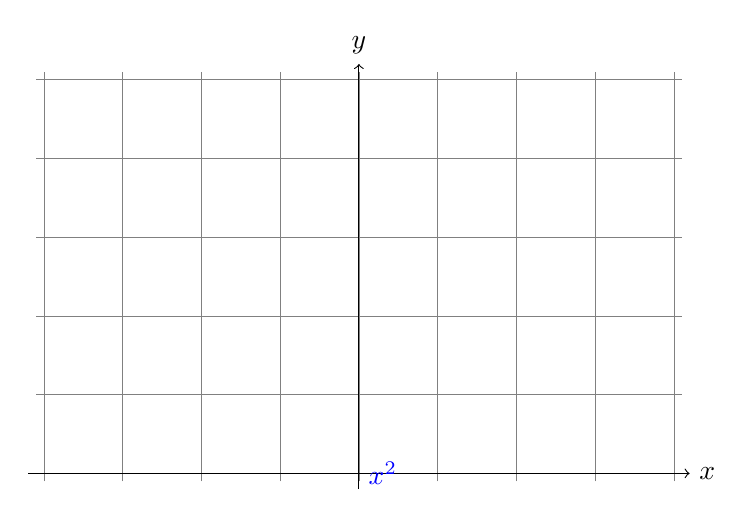
\begin{tikzpicture}[domain=-3.15:3.15]
    \draw[very thin,color=gray] (-4.1,-0.1) grid (4.1,5.1);
    \draw[->] (-4.2,0) -- (4.2,0) node[right] {$x$};
    \draw[->] (0,-0.2) -- (0,5.2) node[above] {$y$};
    \draw[color=blue] plot[id=sin] function{0.5*x**2} 
        node[right] {$x^2$};
    \end{tikzpicture}
    \caption{Parabel}
    \label{fig:my_label}
\end{figure}

\noindent Die Funktion, die wir hier sehen, heißt \textbf{Parabel}. Sie ist standardmäßig nach oben geöffnet und hat ihren tiefsten Punkt (\textbf{Scheitelpunkt}) für den Wert $x=0$. Das können wir einfach begründen: Wenn wir für $x$ eine beliebige Zahl einsetzen, wird $x^2$ niemals negativ, denn Quadrate sind immer positiv. Wenn wir betragsmäßig größere Werte für $x$ einsetzen (also egal, ob positiv oder negativ), erhalten wir auch für das Quadrat größere Werte. Die Funktion wächst also in beide Richtungen, wenn wir vom Scheitelpunkt ausgehen.

Uns interessiert nun, ob wir diese Form immer erhalten, wenn wir eine quadratische Funktion zeichnen.

\begin{definition}
Eine quadratische Funktion von $x$ heißt in \textbf{Scheitelpunktform}, wenn sie der Form $(x-x_S)^2+y_S$ ist, $x_S,y_S\in\mathbb{R}$.
\end{definition}
Die Scheitelpunktform ist für uns sehr hilfreich, da wir an ihr direkt die Koordinaten des Scheitepunkts $S$ der Parabel ablesen können: $S=(x_S,y_S)$. Das Quadrat kann wieder minimal den Wert 0 annehmen.
\begin{theorem}
Jede quadratische Funktion $x^2+bx+c$ kann in die Scheitelpunktform $(x+x_S)^2+y_S$ umgeformt werden, wobei $x_S=\frac{b}{2}, y_S=c-\Big(\frac{b}{2}\Big)^2$.
\end{theorem}
\begin{proof}
Sei eine quadratische Funktion $x^2+bx+c$ gegeben. Wir formen diese Funktion nun schrittweise in Scheitelpunktform um (wieder mit quadratischer Ergänzung):
\begin{equation*}\begin{split}
    x^2+bx+c&=x^2+bx\underbrace{+\Big(\frac{b}{2}\Big)^2-\Big(\frac{b}{2}\Big)^2}_{=0}+c\\
    &=\Big(x+\underbrace{\frac{b}{2}}_{=:x_S}\Big)^2\underbrace{-\Big(\frac{b}{2}\Big)^2+c}_{=:y_S}\\
    &=(x+x_S)^2+y_S
\end{split}\end{equation*}
\end{proof}
Daraus folgt ziemlich direkt, dass wir für beliebige quadratische Gleichungen Parabeln erhalten. Wir können nämlich immer eine Scheitelpunktform erhalten. Also bekommen wir immer einen Scheitelpunkt, von dem aus unsere Funktion in beide Richtungen wächst. Und genau das ist eine Parabel.

Um unser Verständnis für quadratische Gleichungen weiter zu verbessern, schauen wir uns nun Zusammenhänge zwischen der Form der Parabel und der Gleichung an. Dann werden wir auch geometrisch verstehen, warum quadratische Gleichungen manchmal keine, manchmal eine und manchmal zwei Lösungen besitzen.

\end{document}